% !TEX root = ../../../main.tex
% 来源：中学数学实验教材·第三册（高中数学）
% 章节：任意角的三角函数 / 弧和角的概念及其度量
% 原始文件：6.tex，行 26-52
% 类型：tikz
% ---
        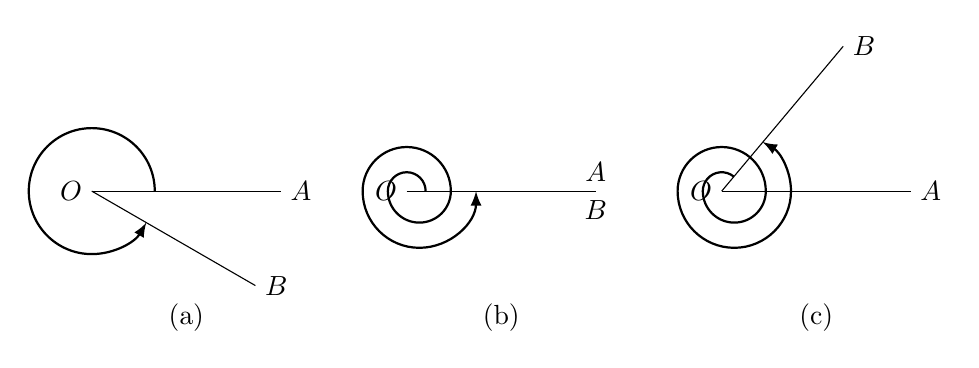
\begin{tikzpicture}[>=latex, scale=.8]
            \begin{scope}
            \draw (0,0)node[left]{$O$}--(3,0)node[right]{$A$};
            \draw (0,0)--(-30:3) node [right]{$B$};
        \draw[->, thick] (1,0) arc (0:360-30:1);
        \node at (1.5,-2){(a)};
    \end{scope}
    \begin{scope}[xshift=5cm]
            \draw (0,0)node[left]{$O$}--(3,0)node[above]{$A$};
          \node at   (3,0)[below]{$B$};
        \draw[thick] (.3,0) arc (0:180:.3);
        \draw[thick] (-.3,0) arc (180:360:.5);
        \draw[thick] (.7,0) arc (0:180:.7);
        \draw[thick,->] (-.7,0) arc (180:360:.9);

        \node at (1.5,-2){(b)};
    \end{scope}
    \begin{scope}[xshift=10cm]
        \draw (0,0)node[left]{$O$}--(3,0)node[right]{$A$};
        \draw (0,0)--(50:3) node [right]{$B$};
        \draw[thick] (50:.3) arc (50:180:.3);
        \draw[thick] (-.3,0) arc (180:360:.5);
        \draw[thick] (.7,0) arc (0:180:.7);
        \draw[thick,->] (-.7,0) arc (180:360+60:.9);
    \node at (1.5,-2){(c)};
\end{scope}
        \end{tikzpicture}
